\documentclass[conference]{IEEEtran}
\IEEEoverridecommandlockouts

\usepackage{cite}
\usepackage{amsmath,amssymb}
\usepackage{graphicx}
\usepackage{booktabs}
\usepackage{textcomp}
\usepackage{xcolor}
\usepackage{url}
\usepackage[hidelinks]{hyperref}

\def\BibTeX{{\rm B\kern-.05em{\sc i\kern-.025em b}\kern-.08em T\kern-.1667em\lower.7ex\hbox{E}\kern-.125em X}}

\begin{document}

\title{Anticipating Dashcam Collisions: Do Learned Temporal Features Beat Motion Cues?}

\author{\IEEEauthorblockN{Muhammad Hoosen (2552770) \and Rameez Atif (2612521)}
\IEEEauthorblockA{COMS4036A Computer Vision, University of the Witwatersrand\\
Code: \url{https://github.com/RameezAtif/nexar-collision-prediction}}}

\maketitle

\begin{abstract}
Can a collision be anticipated from dashcam video before it happens, and does learned temporal modelling help beyond simple cues?
On 1,500 Nexar dashcam videos we compare a naive predictor, optical-flow statistics with logistic regression, and frozen ResNet-18 features with an LSTM,
at 0.5, 1.0 and 1.5\,s before the annotated event, under one video-level split.
The CNN+LSTM reaches average precision (AP) 0.762, 0.749 and 0.675, against 0.575, 0.576 and 0.569 for optical flow (chance 0.5), and degrades as the horizon grows.
However, a classifier on a \emph{single frame} matches it (0.759, 0.752, 0.709), so we cannot show that temporal modelling adds anything.
A single frame taken more than 3\,s before the event already gives AP $\approx$ 0.70, and the two classes occupy disjoint video-id blocks,
so we read the model as recognising high-risk scenes rather than detecting imminent collisions.
Choosing the training epoch on the evaluation videos, as our first experiment did, inflated AP by up to 0.07.
\end{abstract}

\section{Problem}
Collision-warning systems only help if they react \emph{before} an impact. We ask two questions on dashcam video:
(1)~how does prediction quality change as the warning horizon, the time to event (TTE), grows from 0.5 to 1.5\,s; and
(2)~does a learned temporal model beat classical motion cues? Our hypothesis, fixed in the proposal, was that performance falls with TTE but the learned model degrades \emph{more slowly}
than a motion baseline. We call the project a success if the learned model beats optical flow in AP at every TTE with a confidence interval that excludes zero, \emph{and} the gap widens with TTE;
we also probe \emph{what} the model keys on.
Accident anticipation from dashcam video was introduced with attention-based recurrent models~\cite{chan2016anticipating}; our study uses the Nexar benchmark~\cite{moura2025nexar}
and deliberately keeps the models simple so that the comparison is controlled rather than state of the art.

\section{Data}
\textbf{Dataset and licence.} We use the Nexar Dashcam Collision Prediction dataset~\cite{moura2025nexar}: 1,500 labelled training videos of about 40\,s (750 collision or near-collision, 750 normal driving).
Collision videos carry the time of the event and an annotated alert time (mean lead about 1.6\,s). On a 431-video sample we measured every video at 1280$\times$720 and about 30 fps.
The dataset is released under the Nexar open data licence, which allows free use, copying and redistribution with attribution to Nexar Inc.\ and the copyright notice retained, and prohibits resale,
re-identifying people or vehicles, weapons use and systems intended to cause harm. We use the data for research only, attempt no re-identification, and redistribute no videos
(the repository holds labels, clip windows and derived features, with attribution).

\textbf{Split and clips.} The split is made at video level \emph{before} any clip is cut: 1,200 training and 300 held-out videos, stratified 50/50 (seed 42), with zero overlap checked.
For a collision video with event time $t_e$ and a chosen TTE, the prediction time is $t_p=t_e-\mathrm{TTE}$ and the input is 16 frames sampled uniformly from the 2\,s ending at $t_p$;
a check confirms no sampled frame lies after $t_p$. For a normal video there is no event, so $t_p$ is drawn once (seeded) from the empirical distribution of the collision prediction times,
so that clip position in the video is not a shortcut; a position-only classifier scores AUC 0.50--0.53, as intended. One collision video was too short for the window at TTE 1.5\,s and is excluded there (1,199 training clips).
All models use exactly these saved clips. The 300 held-out videos serve as our test set: in the final protocol they never influence epoch selection or tuning (Fig.~\ref{fig:clips}).

\begin{figure}[t]
\centering
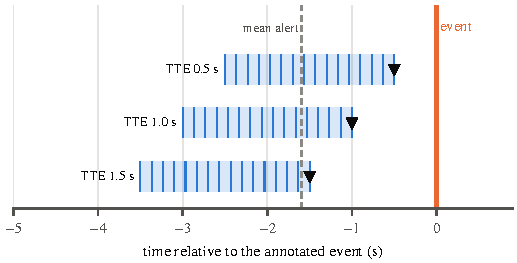
\includegraphics[width=\columnwidth]{figures/fig_clips.pdf}
\caption{Clip construction for the three horizons. Each clip is the 2\,s ending at $t_p=t_e-\mathrm{TTE}$, sampled at 16 frames (ticks); triangles mark $t_p$. The dashed line is the mean annotated alert time (1.6\,s before the event).}
\label{fig:clips}
\end{figure}

\section{Method}
\textbf{Model 0 (naive).} Predict the positive class for every clip; AP equals the 0.5 prevalence.

\textbf{Model 1 (classical motion).} Farneb\"ack dense optical flow~\cite{farneback2003} between consecutive sampled frames (15 pairs, about 0.13\,s apart); per pair the mean and standard deviation of the horizontal and vertical flow and of the magnitude, and the maximum magnitude;
these 7 statistics are summarised over pairs by mean, standard deviation and maximum (21 features), then standardised and fed to logistic regression.

\textbf{Model 2 (learned).} A frozen ImageNet ResNet-18~\cite{he2016resnet} gives a 512-d vector per frame (16$\times$512 per clip), cached once. A one-layer LSTM~\cite{hochreiter1997lstm} (128 units) reads the sequence in order, and its final state feeds a linear layer
(Adam, learning rate $10^{-3}$, batch 32, 10 epochs, BCE loss; one model per TTE).

\textbf{Temporal ablation.} On the \emph{same} features we test whether order matters: the last frame only; the mean of the 16 frames (no order); an LSTM trained and tested on shuffled frames; and the trained LSTM given shuffled frames at test time.

\begin{table}[t]
\caption{What we wrote and what we reused.}
\label{tab:reuse}
\centering\footnotesize
\begin{tabular}{@{}p{0.46\columnwidth}p{0.46\columnwidth}@{}}
\toprule
\textbf{Reused (not ours)} & \textbf{Written by us} \\
\midrule
Nexar videos and labels; ImageNet ResNet-18 weights (torchvision); Farneb\"ack flow (OpenCV~\cite{bradski2000opencv}); LSTM, Adam (PyTorch~\cite{paszke2019pytorch}); logistic regression, AP/AUC (scikit-learn~\cite{pedregosa2011sklearn}); IEEEtran class
& Video-level split, TTE clip sampler and leakage checks; negative sampling; flow-statistic features; feature caching, training and evaluation code; the ablation variants; bootstrap and permutation analyses; failure and id-block analyses; all notebooks and scripts in the repository \\
\bottomrule
\end{tabular}
\end{table}

\section{Experiment and Baselines}
All models share the split, clips, TTEs and metrics. The primary metric is AP (area under the precision--recall curve); we also report recall at a false-alarm rate of at most 10\% of normal clips, since false alarms matter for warning systems.
Each learned variant is trained with 5 seeds (42--46). The epoch is chosen by AP on a stratified 20\% of the \emph{training} videos, never on the test videos, and each trained model is scored once on the test set.
We quote mean $\pm$ standard deviation over seeds, which reflects training noise only; because 300 test clips are few, comparisons use a paired bootstrap (2,000 resamples of the test clips, applied to seed-averaged predictions)
that scores both models on the same resampled clips~\cite{efron1979bootstrap}. Baselines are Models 0 and 1; the single-frame, mean-pool and shuffled variants are controls for Model 2.

\begin{table*}[t]
\caption{Test results (300 held-out videos): mean $\pm$ std over 5 seeds. Optical flow and naive are deterministic. Naive recall at the false-alarm limit is the chance value.}
\label{tab:main}
\centering\footnotesize
\begin{tabular}{@{}lcccccc@{}}
\toprule
 & \multicolumn{3}{c}{AP} & \multicolumn{3}{c}{Recall at FPR $\leq 10\%$} \\
\cmidrule(lr){2-4}\cmidrule(lr){5-7}
Model & 0.5\,s & 1.0\,s & 1.5\,s & 0.5\,s & 1.0\,s & 1.5\,s \\
\midrule
Naive (Model 0) & 0.500 & 0.500 & 0.500 & 0.10 & 0.10 & 0.10 \\
Optical flow (Model 1) & 0.575 & 0.576 & 0.569 & 0.17 & 0.15 & 0.21 \\
CNN+LSTM (Model 2) & 0.762\,$\pm$\,0.019 & 0.749\,$\pm$\,0.011 & 0.675\,$\pm$\,0.021 & 0.38\,$\pm$\,0.03 & 0.43\,$\pm$\,0.02 & 0.30\,$\pm$\,0.03 \\
\bottomrule
\end{tabular}

\end{table*}

\begin{figure*}[t]
\centering
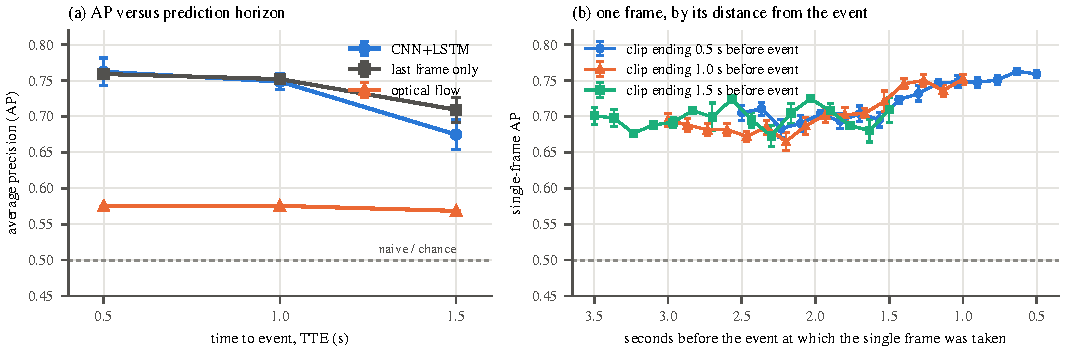
\includegraphics[width=\textwidth]{figures/fig_main.pdf}
\caption{(a) AP versus time to event; error bars are $\pm$1 std over seeds; the dotted line is chance. (b) AP of a classifier trained on a single frame, by how many seconds before the event that frame was taken
(the three curves are the three clip definitions). Test set, 5 seeds.}
\label{fig:main}
\end{figure*}

\section{Results}
\textbf{Learned features beat motion cues.} Table~\ref{tab:main} and Fig.~\ref{fig:main}a show the CNN+LSTM above optical flow at every horizon, by $+0.197$, $+0.180$ and $+0.117$ AP
(95\% CIs $[0.111,0.266]$, $[0.103,0.251]$, $[0.032,0.192]$, all excluding zero). At a 10\% false-alarm limit it recovers 0.38, 0.43 and 0.30 of collisions against 0.17, 0.15 and 0.21 for flow (chance 0.10).
Optical flow is only slightly above chance everywhere.

\textbf{Degradation, and the hypothesis.} The CNN+LSTM loses 0.086 AP from 0.5 to 1.5\,s (95\% CI $[0.030,0.138]$); the 0.5 to 1.0\,s drop (0.016, $[-0.021,0.055]$) is not distinguishable from zero.
Optical flow is flat (0.007, $[-0.052,0.063]$), but only because it sits near chance, so there is little to lose. The hypothesis that the learned model degrades more slowly than flow is therefore \emph{not supported}.

\textbf{Temporal modelling is not demonstrated.} Table~\ref{tab:ablation} and Fig.~\ref{fig:paired} show that a classifier on the last frame alone performs as well as the LSTM at 0.5 and 1.0\,s (AP differences $+0.009$ $[-0.008,0.026]$ and $+0.002$ $[-0.018,0.023]$)
and better at 1.5\,s ($-0.025$, $[-0.044,-0.001]$ in favour of the single frame). Order-free mean-pooling and an LSTM trained on shuffled frames are within noise of the LSTM at all three horizons.
Shuffling frames only at test time costs the trained LSTM 0.031 $[0.008,0.057]$ and 0.023 $[0.003,0.043]$ AP at 0.5 and 1.0\,s, so it uses a little order, but a model that never sees order does as well.
The advantage over optical flow therefore comes mainly from the pretrained visual features.

\begin{table}[t]
\caption{Temporal ablation (AP, mean $\pm$ std over 5 seeds). $^{\dagger}$: the paired 95\% CI of the difference to CNN+LSTM excludes zero.}
\label{tab:ablation}
\centering\footnotesize
\begin{tabular}{@{}lccc@{}}
\toprule
Variant (same ResNet-18 features) & 0.5\,s & 1.0\,s & 1.5\,s \\
\midrule
Last frame only & 0.759\,$\pm$\,0.005 & 0.752\,$\pm$\,0.007 & 0.709\,$\pm$\,0.018$^{\dagger}$ \\
Mean-pool, no order & 0.737\,$\pm$\,0.007 & 0.725\,$\pm$\,0.008 & 0.707\,$\pm$\,0.004 \\
LSTM, shuffled train+test & 0.736\,$\pm$\,0.012 & 0.719\,$\pm$\,0.017 & 0.709\,$\pm$\,0.017 \\
LSTM, shuffled at test only & 0.728\,$\pm$\,0.013$^{\dagger}$ & 0.725\,$\pm$\,0.014$^{\dagger}$ & 0.676\,$\pm$\,0.013 \\
CNN+LSTM (frame order kept) & 0.762\,$\pm$\,0.019 & 0.749\,$\pm$\,0.011 & 0.675\,$\pm$\,0.021 \\
\bottomrule
\end{tabular}

\end{table}

\begin{figure}[t]
\centering
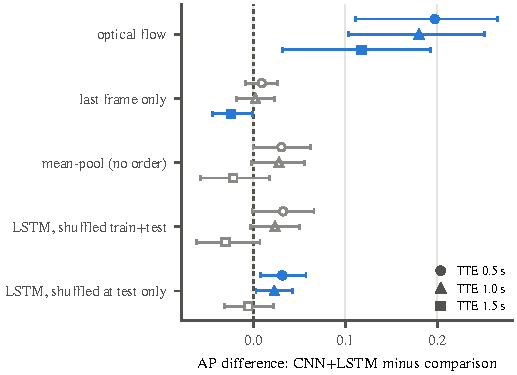
\includegraphics[width=\columnwidth]{figures/fig_paired.pdf}
\caption{Paired AP difference, CNN+LSTM minus each comparison, with 95\% bootstrap CIs. Filled: the CI excludes zero; hollow: it does not. Right of zero favours CNN+LSTM.}
\label{fig:paired}
\end{figure}

\section{Failures and Limitations}
\textbf{The signal is mostly static.} A single frame taken 3\,s or more before the event already gives AP 0.69 (0.68--0.70 across positions); frames within about 1.2\,s of the event raise it only to about 0.75 (Fig.~\ref{fig:main}b).
There is a hazard-related component (Fig.~\ref{fig:alert}): collision clips that end \emph{after} the annotated alert are ranked above normal clips better (CNN+LSTM AUC 0.77, 0.76, 0.72 at 0.5, 1.0, 1.5\,s) than clips ending \emph{before} it
(0.57, 0.66, 0.62; $n$ = 9, 46, 82), though both are above chance. Of the 300 test videos, 71 are wrong at every horizon (36 false alarms, 35 misses).
We inspected 12 of them: the false alarms are mostly dense night traffic with a vehicle close ahead, the misses mostly rain, glare or empty road. This is a qualitative impression, not a result.

\begin{figure}[t]
\centering
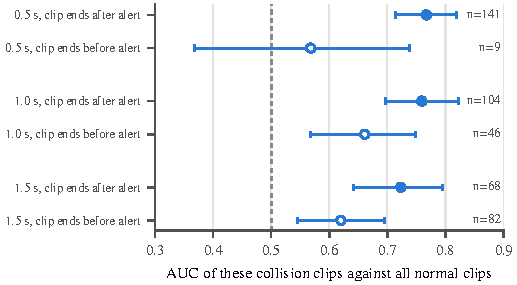
\includegraphics[width=\columnwidth]{figures/fig_alert.pdf}
\caption{CNN+LSTM: AUC of collision clips against all normal clips, split by whether the clip ends before or after the annotated alert (filled: after; hollow: before), with 95\% bootstrap CIs and the number of collision clips. The single-frame model behaves the same way.}
\label{fig:alert}
\end{figure}

\textbf{A dataset-structure caveat.} Every collision video has id $\le$1039 and every normal video id $\ge$1040, so the id alone separates the classes. No model sees the id, but the blocks may differ in recording conditions.
On a 431-video sample we found no difference in resolution, frame rate, duration, brightness or overlay, and these properties together predict the class at AUC 0.58, within what shuffled labels reach (mean 0.49, maximum 0.61).
The features do show a trace of id order: the collision score drifts down with id inside the collision block (Spearman $-0.13$, permutation $p=0.0005$) and class separation is weaker near the id boundary (AUC 0.59 within 100 ids of it, 0.73 farther away).
We did not test scene content (location, season, traffic), so we describe the model as separating the two video groups, most plausibly by recognising high-risk scenes, and not as detecting imminent collisions.

\textbf{Protocol pitfalls we hit.} Our first CNN+LSTM experiment kept the epoch with the best AP on the evaluation videos and reported that score (AP 0.793, 0.774, 0.739).
Training on the full training set for a fixed 10 epochs, with no selection, gives 0.754, 0.753, 0.676, so the selection inflated AP by about 0.04, 0.03 and 0.07, most at 1.5\,s, which also flattened the apparent degradation.
Holding out 20\% of training videos instead costs almost nothing (0.762, 0.749, 0.675; Table~\ref{tab:selection}), so we report that protocol. Validation AP peaks after only 3--5 epochs, so a fixed 10 epochs is slightly conservative.

\begin{table}[t]
\caption{CNN+LSTM AP on the test videos under different epoch-selection protocols (single seed for the first row).}
\label{tab:selection}
\centering
\scriptsize
\setlength{\tabcolsep}{2.5pt}
\begin{tabular}{@{}lccc@{}}
\toprule
CNN+LSTM, how the epoch is chosen & 0.5\,s & 1.0\,s & 1.5\,s \\
\midrule
Best epoch on the test videos (first run) & 0.793 & 0.774 & 0.739 \\
Same, mean of 5 seeds & 0.793 & 0.780 & 0.742 \\
Fixed 10 epochs, no selection & 0.754\,$\pm$\,0.015 & 0.753\,$\pm$\,0.009 & 0.676\,$\pm$\,0.021 \\
Epoch chosen on held-out training videos & 0.762\,$\pm$\,0.019 & 0.749\,$\pm$\,0.011 & 0.675\,$\pm$\,0.021 \\
\bottomrule
\end{tabular}

\end{table}

\textbf{Other limits.} There is no separate untouched test set: the 300 videos were used for earlier choices (the scaled flow variant, about 0.01 AP; the unscaled variant did not converge). With 300 clips an AP has a 95\% interval of about $\pm$0.07, so differences near 0.03 are within noise.
We use one frozen backbone and one clip design, and the flow baseline uses frames 0.13\,s apart rather than adjacent frames, so classical motion cues may be underestimated.

\section{Next Steps}
(i)~Compare the two id blocks on scene content and recording metadata with all 1,500 videos, and evaluate on a split that holds out id ranges. (ii)~Choose the epoch count and regularisation by nested cross-validation on training videos,
since the models overfit after a few epochs. (iii)~Compute flow between adjacent frames and add a fine-tuned or two-stream model, to test whether temporal information helps once the static shortcut is weaker.
(iv)~Add multiple seeds and intervals to every ablation and calibrate an operating threshold for a fixed false-alarm budget.

\section*{Use of AI Tools}
% CONFIRM with Rameez before submission: whether AI tools were also used for notebooks 01--05 and his analysis notebook, and that the course AI policy allows this level of use.
We used Claude Code (Anthropic) during the later stages of the project. It wrote the analysis notebooks 06--09, the helper scripts in \texttt{tools/}, the report tables and figures script, the README and the experiment log,
and it helped design the controls (single-frame, mean-pool, shuffled order), the bootstrap comparisons and the id-block tests, and drafted this report. It also reviewed the partner's analysis notebook.
The data pipeline and the baseline and CNN+LSTM notebooks (01--05) were written by the group. We ran the code and checked its outputs; reviewing them exposed that our first results used the evaluation videos for epoch selection, and we re-ran the experiments with a clean protocol.
We remain accountable for every line and claim. All numbers in this report are generated from files in the repository (\texttt{README.md}, ``Where each reported number comes from'').

\bibliographystyle{IEEEtran}
\bibliography{refs}

\end{document}
